\section{Economic actions after provenance and feasibility checks}
\label{sec:sol-economic-results}

The games contain substantial acquisition, bargaining, construction and liquidation. They also show why an observed action is an insufficient behavioral label. We describe the opportunities, separate development outcomes by their resolution, and test every elimination against current-debt financing.

\begin{figure}[t]
\centering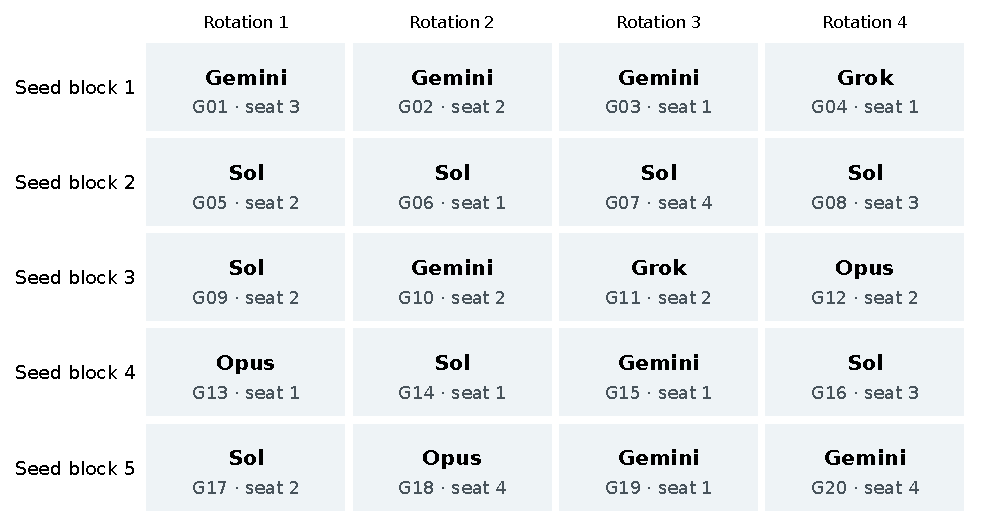
\includegraphics[width=\linewidth]{cohort.pdf}
\caption{Winner and seat in all twenty games. Each row shares an initial seed and contains four cyclic rotations. Sol wins one block from every seat; another block is won from seat 2 by all four configurations. These are descriptive outcomes, not independent trials of a model ranking. Table~\ref{tab:configurations} specifies response conditions.}
\label{fig:cohort}
\end{figure}

\subsection{Acquisition creates unequal opportunities}

The cohort records 475 direct, 72 auction, 207 trade and 397 inherited deed acquisitions, including repeated acquisitions of a deed. Stable transaction boundaries yield 209 completed-group episodes: sixteen by direct purchase, nine by auction, sixty-three by trade and 121 by inheritance. Sixty-nine inherited completions occur at game-ending bankruptcy. They provide no subsequent management opportunity. Treating them as undeveloped investments would invent decisions after play ended.

\begin{table}[t]
\centering\small
\begin{tabular}{lrrrrr}\toprule
Agent & Proposals & Proposing/eligible turns & Share & Intensity & Eligible decisions\\\midrule
Sol & 132 & 83/834 & 10.0\% & 1.59 & 1,133 \\
Gemini & 18 & 16/766 & 2.1\% & 1.12 & 1,001 \\
Opus & 240 & 160/660 & 24.2\% & 1.50 & 1,050 \\
Grok & 136 & 106/676 & 15.7\% & 1.28 & 897 \\
\bottomrule\end{tabular}
\caption{Negotiation initiation. Intensity is proposals per proposing turn. The final column records a different, action-dependent denominator; it is not an additional set of independent opportunities. Rounding uses two-decimal half-even display where applicable. All conditions in Table~\ref{tab:configurations} remain in these configured-system counts.}
\label{tab:negotiation}
\end{table}


The 113 accepted trades complete a color group for neither party in sixty settlements, one party in forty-three, and both parties in ten. In forty-four, the final offer author differs from the thread initiator. Assigning the transferred bundles to the initiator would misattribute those counteroffers. Negotiation also has distinct initiating and responding roles. Gemini initiates eighteen proposals but applies twenty-six acceptances; Opus initiates 240 and applies twenty-nine. Table~\ref{tab:negotiation} reports the propensity to propose on an eligible own turn and proposals per proposing turn. Neither measures agreement quality, and a completion cannot by itself establish which side benefited.

Trade is not necessary for every observed win. G14 Sol and G15 Gemini participate in no accepted trade. In G15, Gemini purchases Tennessee, completes oranges at event 711, and first builds at event 718 in turn 47. Oranges collect \$3,250 in developed rent and trigger the first two eliminations. Inherited browns trigger the last; greens arrive only in the terminal estate. This corrects an earlier research label attributing the trajectory to greens. Figure~\ref{fig:cohort} locates these paths in the full cohort, whose win totals are Sol eight, Gemini seven, Opus three and Grok two. Shared-seed blocks and differing response conditions preclude reading those totals as an intrinsic capability ordering.

\subsection{An unbuilt group need not be a declined investment}

\begin{figure}[t]
\centering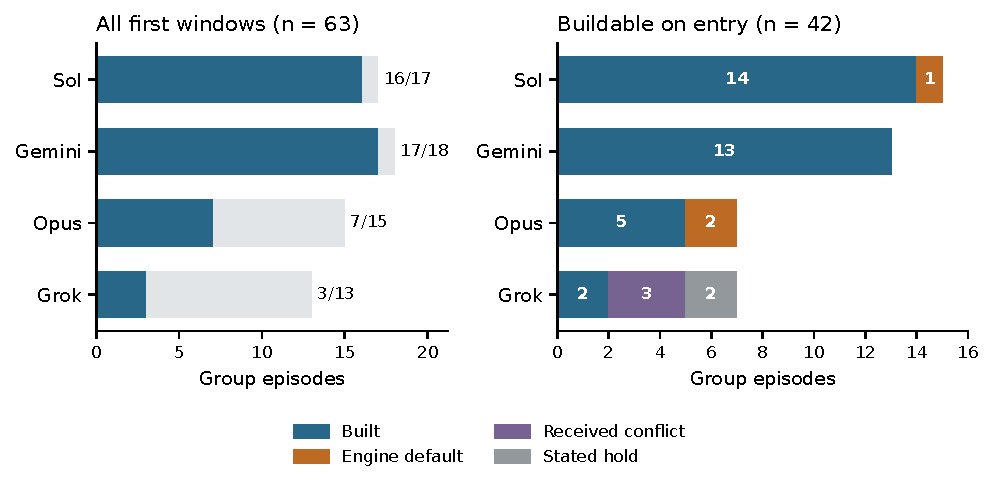
\includegraphics[width=\linewidth]{development.pdf}
\caption{First management after trade completion. Left: construction over all 63 acquired groups, including groups not buildable on entry. Right: the 42 entry-buildable groups by actual resolution. Eight remain unbuilt: three engine defaults, three received END conflicts and two stated holds. A content request need not be executable as encoded. Counts retain each configuration's response condition; they do not measure willingness to invest.}
\label{fig:development}
\end{figure}

All sixty-three trade-completed groups have an observed first management window. Sol builds sixteen of seventeen, Gemini seventeen of eighteen, Opus seven of fifteen, and Grok three of thirteen. The twenty unbuilt groups split into nine never buildable during that window, four engine defaults, four received END conflicts and three other valid END records. All nine never-buildable groups belong to Opus or Grok. The whole-window outcome thus combines acquisition, financing access and resolution, rather than measuring a common choice to build.

Conditioning on the forty-two groups buildable on entry yields thirty-four built groups. The eight residuals are three defaults, three conflicts and two stated holds (Figure~\ref{fig:development}). The difference from the whole-window decomposition comes from groups that become buildable only later. In one conflict the content requests finance; in another its construction request is uneven as encoded. Calling these lost executable builds would overstate the evidence. Likewise, a valid END without a detected conflict does not establish a coherent reserve policy.

Across 1,225 management menus listing the construction tool, 663 applied actions are END (Table~\ref{tab:end-provenance}). Sixty-six are deterministic defaults after failed attempts; twenty-four are selected valid calls whose names conflict with a named content action. The remaining 573 have no detected name conflict. That category includes absent or unparseable content and is not a count of verified choices to hold. Tool availability also does not prove that a particular allocation was affordable. This census measures provenance, not opportunity quality or latent intention.

\begin{table}[t]
\centering\small
\begin{tabular}{lrrrrr}\toprule
Configuration & Tool-listed & END & Default & Name conflict & No detected conflict\\\midrule
Sol & 399 & 236 & 4 & 0 & 232 \\
Gemini & 330 & 144 & 1 & 0 & 143 \\
Opus & 223 & 104 & 61 & 0 & 43 \\
Grok & 273 & 179 & 0 & 24 & 155 \\
\midrule Total & 1,225 & 663 & 66 & 24 & 573\\\bottomrule
\end{tabular}
\caption{Every applied END on a management menu listing construction. Categories partition ENDs, not all listed menus. A default is engine-authored; a conflict is disagreement between selected content and received call names. The remainder includes empty or unparseable content and matching names, not verified reserve choices. Sol and Gemini's selected content fields are all empty; 42 of 43 nondefault Opus ENDs use action-only recovery. Grok uses required tool selection. These observation conditions prevent comparing the last two columns as error or intention rates.}
\label{tab:end-provenance}
\end{table}


For Opus, sixty-one of 104 such ENDs are defaults. All sixty-one attempted purchase multisets execute at the same historical state after splitting count-valued entries into atomic purchases and ordering those purchases legally. Every original encoding remains invalid. Sixty chains contain a refusal followed by an invalid action-only retry; G2 d129 has the invalid attempt before the refusal. The exhausted resolution policy then applies END. The observed non-build is an execution outcome, not evidence that the configuration preferred cash to its submitted allocation.

\begin{table}[t]
\centering\small
\begin{tabular}{lrrrrr}\toprule
Agent & Rejections & Some build & Same multiset & Changed multiset & Default\\\midrule
Sol & 29 & 25 & 20 & 5 & 4 \\
Gemini & 19 & 18 & 6 & 12 & 1 \\
Opus & 61 & 0 & 0 & 0 & 61 \\
Grok & 5 & 5 & 5 & 0 & 0 \\
\bottomrule\end{tabular}
\caption{Decisions with an uneven-intermediate-building rejection, followed through resolution. ``Some build'' means construction was applied in the same decision, not that the requested allocation or quantity was preserved. Opus's action-only recovery has already used the retry budget. Atomic expansion and ordering of the identical purchases execute all 61 defaulted Opus multisets in exact-prefix tests; the original encodings were invalid.}
\label{tab:recovery}
\end{table}


The portable audit checks all sixty-six construction defaults and every recorded attempt. All seventy well-formed targets are invalid as encoded. Sixty-three execute after atomic expansion and reordering; seven cost more than current cash. One further target is malformed, and sixty-one attempts contain no parseable target. At decision level, sixty-three of sixty-six defaults contain at least one reachable submitted target: sixty-one Opus, one Sol and one Gemini. All sixty-six allow some legal construction, a weaker claim than reaching the submitted target.

Successful retry also needs a precise endpoint. Following an uneven-building rejection, the original purchase multiset is preserved in 20/25 Sol, 6/18 Gemini and 5/5 Grok decisions that end in construction. A different legal build is recovery of action validity, not necessarily of the requested allocation. G2 d243's seven-house target can execute and leave \$208; the actual retry and next decision buy six houses and leave \$358. G14 d145--148 eventually attains its original eight-house target within the same turn. Per-decision preservation and same-turn attainment differ.

There are also checked holds. G3 d176 is a valid Opus action-only END with \$204 and an explicit preference for reserves over a legal \$150 house; no fallback occurs. G1 d426 is a consistent Grok END with \$488 and one house on each yellow. An extra Atlantic house is legal but reduces subsequent liquidation capacity by its \$75 purchase-to-resale loss. These support expressed reserve preferences without establishing optimality. A refusal condition alone cannot classify the next END as engine-authored.

\subsection{A bankruptcy need not imply an unpayable current debt}

\begin{figure}[t]
\centering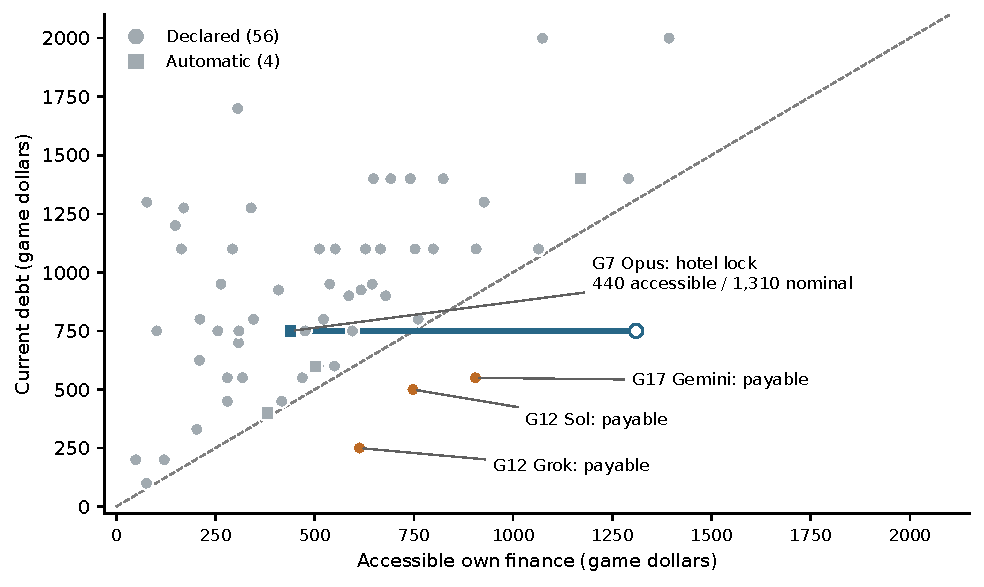
\includegraphics[width=\linewidth]{financing.pdf}
\caption{All sixty eliminations. Fifty-six cannot pay even under the full upper bound, three have a tested own-action payment route, and one is restricted by hotel liquidation. The G7 segment joins accessible \$440 to nominal \$1,310 against \$750 owed. Circles mark declarations and squares automatic eliminations. These classify the current debt without outside assistance, optimality or an alternate-winner claim.}
\label{fig:financing}
\end{figure}

The complete elimination census includes fifty-six declarations and four automatic bankruptcies after mortgages. In fifty-six cases, the upper bound in Equation~\ref{eq:sol-upper} is below the debt, so no permitted own-asset financing sequence can pay. Three cases have legal payment witnesses. The remaining case has sufficient nominal assets but no legal access to enough of them. These conclusions cover all sixty eliminations, rather than selecting only declarations with financing options listed.

\begin{table}[t]
\centering\small
\begin{tabular}{llrrp{0.35\linewidth}}
\toprule
Case & Agent & Debt & Nominal upper & Certificate at the recorded prefix\\
\midrule
G12 d190 & Sol & \$500 & \$748 & Sales and mortgages pay; \$38 remains.\\
G12 d249 & Grok & \$250 & \$613 & Five house sales pay; \$43 remains.\\
G17 d234 & Gemini & \$550 & \$905 & Sales and mortgages pay; \$180 remains.\\
G7 d339 & Opus & \$750 & \$1,310 & Exhaustive current financing reaches only \$440.\\
\bottomrule
\end{tabular}
\caption{The four cases not ruled out by the nominal bound. Payment witnesses are routes executed by the portable audit; they are not minimal and need not realize the upper bound. Earlier checked routes retain \$8 and \$155 in the first and third cases by mortgaging different collateral.}
\label{tab:sol-financing}
\end{table}

The payable eliminations do not share a reasoning mechanism. Sol's G12 d190 account omits red collateral unlocked by house sales. Gemini's G17 d234 account similarly understates accessible collateral. Grok's G12 d249 instead contains a received declaration alongside content requesting a house sale and final explanations opposing bankruptcy. Five legal sales pay without a mortgage. This establishes a financing-feasible applied elimination, not deliberate surrender or a uniform omitted-mortgages error.

G7 d339 is a different negative case. Opus has \$390, a clear Oriental mortgage worth \$50, and pinks at four houses, four houses and a hotel. With no bank houses, the hotel cannot be downgraded; even-selling prevents a lower sibling sale. No building-sale action is offered. The only financing action, mortgaging Oriental, triggers automatic bankruptcy at \$440 against \$750 owed. Exhausting this one-action continuation proves the local lock despite \$1,310 nominal value. Earlier opportunities to release houses are different intervention states, not an escape available at this debt decision.

Actual G20 d327--336 supplies a positive contrast: \$700 salvage and \$665 mortgages from \$49 cash pay \$1,400 and retain \$14. At G16 d602, extensive liquidation instead reaches \$1,393 against \$2,000. The agent's note states the correct total; an earlier research label omitted \$160 of unlocked collateral. Applying the same financing test to agents and researchers prevents both a false failure label and an invented escape route.

\subsection{Consequences retain ownership and exposure}

The 103 spending units incur \$103,450 of construction expenditure and collect \$93,000 in whole-game paid developed rent, \$92,550 after first own spending. Forty collect zero developed rent, and twenty-six of those also trigger no creditor elimination. These are observed cash flows, not failed-investment counts: inherited development, terminal demands, salvage and remaining exposure differ. Even the post-first-spend window can precede later own expenditure. Appendix~\ref{app:economic-detail} retains the accounting and figure rather than treating receipt-to-spending ratios as ROI.

Inheritance connects individual actions to the wider trajectory. Winners hold fifty-eight spending units; thirty-four contain inherited deeds at first own spending, but only thirty first become complete through an estate. The eventual winner is creditor in 54/60 eliminations, including 35/40 nonterminal eliminations. These describe realized concentration under intact creditor inheritance, not a causal advantage estimated by this cohort. The social analysis next asks what players said about such consequences and what their counterparties received.
